\section{Description of the optimization framework}\label{framework}
A fully automated and modular optimization framework was developed to solve the optimization problems in this work. The proposed framework is composed of several components, which are described in detail below:

\begin{enumerate}
	\item \textbf{Optimization}:  
	The first component encompasses the optimization method, which governs the entire process. In this part, the optimization problem is defined along with any required constraints.
	
	In this study, we use the Nelder-Mead method, implemented in Python specifically for this work and detailed in Appendix~\ref{appendix B}. Additionally, the framework includes the MADS method (see Section~\ref{direct-search}), implemented in the open-source \texttt{NOMAD} library \cite{nomad} in C++. For handling constraints in both the Nelder-Mead and MADS methods, we use the extreme barrier function.
	
	\item \textbf{Geometry Generation}:  
	The optimization parameters, updated at each iteration, are passed to the geometry generator. For generating the geometries used in numerical simulations, we use the \texttt{meshgen} package detailed in Chapter~\ref{geometry}.
	
	\item \textbf{Numerical Simulation}:  
	The final component of the optimization framework is the numerical solver, which evaluates the objective function based on the generated geometry. Numerical simulations are performed using the LBM, which is described alongside additional implementation details in Chapter~\ref{lbm}.
\end{enumerate}

The interconnection of these components within the optimization framework is schematically illustrated in Figure~\ref{fig:framework}.


\begin{figure}[H]
	\vspace{5mm}
	\centering
	\includegraphics[width=0.95\textwidth]{figures/framework-en.pdf}
	\vspace{5mm}
	\caption{Schematic representation of the modular optimization framework. It consists of three main components: (1) Optimization, which defines the problem and governs the iterative process, (2) Geometry generation, where optimization parameters are translated into geometric models using \texttt{meshgen}, and (3) Numerical simulation, where the objective function is evaluated using the LBM.}
	\label{fig:framework}
	
\end{figure}